\Chapter{Modélisation par les vitesses de dérive}
\chaptermark{Les vitesses de dérive}
\begin{refsection}
Le deuxième chapitre de cette thèse concerne la modélisation du transport
(fortement) magnétisé par une approche basée sur les vitesses de dérive. Cette
méthode, élaborée dans le cadre de la recherche sur la fusion par
confinement magnétique, est implémentée dans TOKAM2D~\cite{Sarazin}, un code 
spécifiquement développé pour caractériser le transport dans le plasma de bord
des tokamaks.

Nous introduisons tout d'abord le code TOKAM2D et les hypothèses sur
lesquelles repose le modèle. Les équations de continuité et de
courant sont ensuites dérivées avec quelques précisions sur les approximations
choisies.
Dans une deuxième partie, nous présentons les évolutions du
modèle et les modifications entreprises sur le code pour lui
permettre décrire le transport dans des conditions caractéristiques aux plasmas
froids. Sont ainsi passées en revues :

\begin{itemize}
  \item l'inclusion de conditions aux limites
perpendiculaires
\item la prise en compte de géométries de champ magnétique complexes
\item l'ajout de l'équation de la
température électronique
\item la construction d'un modèle basé sur les vitesses de dérive pour les plasmas froids
\end{itemize}

Pour le dernier point, les équations sont redérivées en tenant
compte du transport collisionnel avec les neutres. Le modèle intègre de plus des
conditions aux limites de type gaine sur le courant et le flux de particules
dans la direction perpendiculaire au champ magnétique.

\section{Le code TOKAM2D}

\sectionmark{Le code TOKAM2D}
La première année de cette thèse a consisté à utiliser et modifier le
code {TOKAM2D}. Le but était alors de se familiariser avec les
techniques développées pour la modélisation des plasmas
de SOL et les mécanismes du transport magnétisé afin
de pouvoir les appliquer au problème des sources d'ions. 

Le code TOKAM2D est un code fluide, quasineutre, qui décrit le transport
transverse en se basant sur l'approximation des vitesses de dérive (voir §
\ref{Introduction}-\ref{vitessesDerive}). Initialement développé à
l'Institut Méditerranéen Technologique de Marseille (IMTM) pour étudier
la turbulence d'interchange, sa modification pour intégrer un forçage de la turbulence
par un flux au lieu d'un gradient d'équilibre a permis de retrouver le
caractère intermittent du transport et la longueur de décroissance du profil de
densité que l'on mesurait expérimentalement~\cite{SarazinPhD}. L'étude du modèle a
ainsi permis d'améliorer la compréhension du mécanisme de l'instabilité
d'interchange, par la mise en évidence du transport turbulent de type
avalanche. Il a aussi aidé à prouver le déclenchement à seuil de
l'instabilité.

\subsection{Hypothèses du modèle}
Dans les conditions typiques de la SOL, l'utilisation d'un modèle fluide est
justifiée par la forte collisionnalité du plasma. Le libre parcours moyen
$\lambda_{ei}=v_T \nu_{ei}$, de l'ordre du mètre, est très inférieur à la
longueur de connexion parallèle des lignes de champ $L_\para\sim
$~100m.

Le plasma est de plus très magnétisé $B\sim$~1T, les fréquences
caractéristiques du transport transverse sont donc suffisement lentes devant la
fréquence cyclotronique ionique pour nous placer dans le cadre de
l'approche par vitesses de dérive :

\begin{equation}
\omega\ll\omega_c\Leftrightarrow \varepsilon_\omega\equiv\frac{\omega}{\omega_c}\ll 1
\end{equation}

D'un autre côté $\rho\indice{i}$, le rayon de Larmor ionique, d'environ
1mm, est bien supérieur à la longueur de
Debye $\lambda_D$, de l'ordre de 10$^{-5}$~m, ce qui autorise à
considérer le plasma quasineutre dans son ensemble, avec des densités ionique
et électronique équales à $n$.
Le transport est alors décrit à travers l'évolution de la densité
électronique $n$ et du potentiel électrostatique $U$ en résolvant l'équation
de continuité des électrons ainsi que l'équation de conservation du courant. Les
températures électronique
$T_e$ et ionique $T_i$ sont supposées constantes, avec un rapport $\tau=T_i/T_e$.

\begin{figure}[htbp]
\centering
    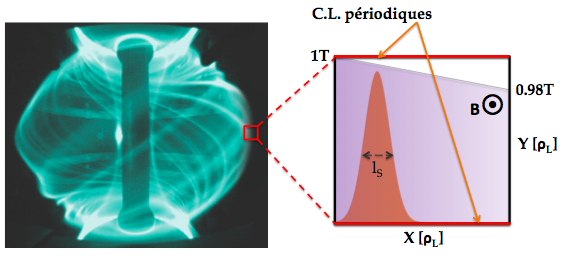
\includegraphics[width=0.8\textwidth]{figures/2-tokamSimDomain.png}
    \caption{La région simulée est située à la frontière du plasma confiné,
    au niveau de la séparatrice, et dans le plan poloïdal médian.}
    \label{2-figTokamGeom}
\end{figure}

L'hypothèse flûte, qui sera développée §\ref{2-flute}, permet enfin de réduire
le problème de trois à deux dimensions.
La figure~\ref{2-figTokamGeom} montre la zone simulée. La SOL est représentée
en géométrie slab, ie. avec $x\equiv(r-a)/\rho_i$ et $y\equiv
a\theta/\rho_i$ les coordonnées transverses, normalisées par le rayon de
Larmor ionique. La séparatrice est modélisée par un flux entrant de particules,
qui sépare la zone simulée en deux régions :

\begin{itemize}
  \item une région stable, ie. où la courbure magnétique est favorable, à gauche
  de la source
  \item une région sujette à l'instabilité d'interchange (côté LFS) à droite
 \end{itemize}
 
Dans la version initiale de TOKAM2D, pour des raisons pratiques, le domaine de
simulation a été choisi bipériodique. 

\subsection{Dérivation des équations}
\subsubsection{Equation de conservation de la matière}
La densité $n$ du plasma est conrôlée par l'équation de continuité des
électrons. L'effet des collisions coulombiennes est pris en compte à travers un
terme diffusif de coefficient $D_\perp\sim eT_\text{e}/m_\text{e}\nu_\text{ei}$
et on note $S$ un terme source modélisant le flux de particules
provenant du plasma de c\oe{}ur. L'équation de continuité s'écrit :

\begin{equation}
\label{2-ContinuiteElectrons}
\partial_t n + \nabla\cdot(n\mathbf{u}) = D_\perp\nabla^2_\perp n + S
\end{equation}

En décomposant la divergence suivant les directions parallèle et
perpendiculaire, et en se souvenant que le flux de matière transverse est
essentiellement issu de l'advection par la vitesse de dérive électrique
(cf.~§\ref{Introduction}-\ref{vitessesDerive}), \eqref{2-ContinuiteElectrons} peut se développer en :

\begin{equation}
\label{2-ContinuiteElectrons2}
\partial_t n + \nabla_\para\cdot(n\mathbf{u}_{\para}) =
\mathbf{u}_E\cdot\nabla_\perp n + D_\perp\nabla^2_\perp n + S
\end{equation}

Le terme d'advection $\mathbf{u}_E\cdot\nabla_\perp
n$ se réécrit en utilisant la notation
du crochet de Poisson $[n,U]=\mathbf{b}.(\nabla_\perp n\times\nabla_\perp U)$.
C'est la forme que prend toute advection d'un champ scalaire par une vitesse de
dérive $\mathbf{v}_\text{D}=\nabla H\times\mathbf{B}/B^2$, où $\nabla H$ est la
force à l'origine de la dérive. L'équation de continuité pour les électrons
s'écrit alors :

\begin{equation}
\label{2-eqContinuiteFinale}
\partial_t n + \nabla_{\para}\cdot(n\mathbf{u}^e_{\para}) =
\frac{1}{B}\left[n,U\right] + D_\perp\nabla^2_\perp n + S
\end{equation}

Le terme non-linéraire $[n,U]$ est l'un des éléments moteur du modèle
d'interchange. Couplant la densité au potentiel électrique, il opère un
transfert d'exitation des composantes radiales des fluctuations à leurs
composantes poloïdales et réciproquement. Les termes de flux parallèle et de
diffusion sont stabilisant, ils tendent à
amortir les fluctuations et donc à homogénéiser le système.

\subsubsection{Equation de conservation du courant}
L'équation de conservation du courant s'obtient en soustrayant l'équation de
continuité des électrons à celle des ions. La vitesse de dérive électrique
$\mathbf{u}_E$, indépendante de la masse et de la charge des particules,
est identique pour les deux espèces et ne transporte donc aucun courant. 
La conservation du courant se résume ainsi à un équilibre entre le courant
parallèle $\mathbf{j}_\para$ et les courants transverses diamagnétique
$\mathbf{j}_*$ et de polarisation $\mathbf{j}_p$ à travers leur
divergences:

\begin{equation}
\label{EqCourant1}
\nabla\cdot\left(\mathbf{j}\right) = 
\nabla\cdot\left(\mathbf{j}_\para+\mathbf{j}_*+\mathbf{j}_p\right)
= 0
\end{equation}

La divergence du courant diamagnétique, dans un plasma isotherme, donne un
crochet de Poisson entre la densité et la courbure du champ magnétique :

\begin{equation}
\nabla\cdot\mathbf{j}_*=
\nabla_\perp\cdot\left(\nabla_\perp\left(
P_i+P_e\right)\times\mathbf{B}/B^2\right) =
T_e(1+\tau)\left[n,B\puissance{-1}\right]
\end{equation}

La vitesse de polarisation étant de plus
proportionnelle à la masse des particules \eqrefp{1-vitessePol}, on ne
retient dans l'expression du courant que la contribution ionique :
\begin{equation}
\mathbf{j}_p\sim\text{e}n\mathbf{u}^i_p=-\frac{nm_\text{i}}{B^2}\frac{\text{d}\nabla_\perp
U}{\text{dt}}
\end{equation}

En exprimant la dérivée totale de
façon eulérienne, la divergence du courant de polarisation devient :
\begin{equation}
\nabla\cdot\mathbf{j}_p\sim\nabla\cdot\left(\text{e}n\mathbf{u}^i_p\right)\equiv
-\nabla_\perp\cdot\left(\frac{nm_\text{i}}{B^2}\left(\partial_\text{t} -
\nu_\perp \nabla_\perp^2 +
\mathbf{u}\cdot\nabla_\perp\right)\nabla_\perp U\right)
\end{equation}
$\nu_\perp$ représentant une viscosité effective du milieu\footnote{L'origine
physique de cette viscosité définie par le coéfficient $nu_\perp$ peut être
rapprochée de la conductivité de Spitzer $\eta\equiv
n_\text{e}e\puissance{2}/m_\text{e}\nu_\text{ei}$, soit encore à une expression
modifiée de la vitesse de dérive électrique
$\mathbf{u}_\text{E}=(1+\rho_\text{L}\puissance{2}/4\nabla\puissance{2})\mathbf{E}\times\mathbf{B}/B\puissance{2}$}.
De manière similaire à \eqref{2-ContinuiteElectrons2}, seule l'advection par la
vitesse de dérive électrique est considérée dans la divergence : 
$\nabla\cdot\left(\mathbf{u}\,\nabla_\perp^2 U\right)
\approx\nabla\cdot\left(\mathbf{u}_E\,\nabla_\perp^2 U\right)$.
En insérant l'expression des dérives, \eqref{EqCourant1} se réécrit :

\begin{equation}\begin{split}
\label{EqCourant2}
\nabla_\para\cdot\mathbf{j}_\para +
T_e(1+\tau)\left[n,B\puissance{-1}\right] + \nabla_\perp\cdot\left(-\frac{nm_\text{i}}{B^2}\left(\partial_\text{t}\nabla_\perp
U - \nu_\perp \nabla_\perp^3 U \right)\right) \\+
\nabla_\perp\cdot\left(-\frac{nm_\text{i}}{B^2}\mathbf{u}_E\cdot\nabla_\perp^2
U\right)=0
\end{split}
\end{equation}

Diverses considérations sur l'importance relative des termes contenus dans
\eqref{EqCourant2} (reliées aux hypothèses d'ordering
et aux variations de champ magnétique) sont développées dans
\cite{SarazinPhD} pour réduire le modèle. Elles conduisent à l'expression
simplifiée de l'équation du courant :

\begin{equation}\begin{split}
\label{2-eqCourantFinale}
\nabla_\para\cdot\mathbf{j}_\para +
T_e(1+\tau)\left[n,B\puissance{-1}\right] =\\
\frac{nm_i}{B^2}\left(\partial_\text{t}\nabla_\perp^2 U - \nu_\perp
\nabla_\perp^4U+
B\puissance{-1}\left[U,\nabla_\perp^2\ U\right]\right)
\end{split}
\end{equation}

\subsection{Normalisation du système}
Pour faire apparaître les grandeurs caractéristiques du système et simplifier
l'écriture des équations, les différents termes sont
maintenant adimensionnées. L'intensité du champ
magnétique $B\indice{0}$ et à la température électronique de référence
$T\indice{0}$ constituent les bases de cet adimensionnement. Le temps est
normalisé à l'inverse de la fréquence cyclotronique ionique :

\begin{equation}
t = \overline{t}\:\omega_c\puissance{-1} =
\overline{t}\:\frac{m_i}{eB\indice{0}}
\end{equation}

Les longueurs et vitesses sont alors logiquement normalisées par le rayon de
Larmor et la vitesse de Bohm :

\begin{eqnarray}
x = \overline{x}\:\rho_L =
\overline{x}\:\frac{m_ic_s}{eB\indice{0}} &
et &
v=\overline{v}\:c_s=\overline{v}\left(\frac{eT\indice{0}}{m_i}\right)^{\text{\textonehalf}}
\end{eqnarray}

Nous définissons de plus les variables adimensionnées du modèle, la densité
$\overline{N}$ et le potentiel électrostatique $\overline \phi$ par :

\begin{eqnarray}
n = n_{\indice{0}}\:\overline{N} & \text{et} & U=\frac{\overline
{\phi}T\indice{0}}{e}
\end{eqnarray}

Avec cette normalisation, on réécrit le système d'équations (
\eqref{2-eqContinuiteFinale}-\eqref{2-eqCourantFinale}) sous la forme :

\begin{equation}
\label{2-eqContinuiteNorm}
\partial_t N +
\frac{\rho\indice{i}}{L_{\para}}\nabla_{\para}\cdot(NM^e_{\para}) =
\frac{1}{B}\left[N,\Phi\right] + D_\perp\nabla^2_\perp N + S
\end{equation}

\begin{equation}\begin{split}
\label{2-eqCourantNorm}
\nabla_\para\cdot(N\mathbf{M}_\para) +
T_e(1+\tau)\left[N,B\puissance{-1}\right] =\\
\frac{N}{B^2}\left(\partial_\text{t}\nabla_\perp^2 U - \nu_\perp
\nabla_\perp^4U+
B\puissance{-1}\left[U,\nabla_\perp^2\ U\right]\right)
\end{split}
\end{equation}

Cette expression fait apparaître la vorticité électrique\footnote{La
vorticité d'un écoulement est généralement définie comme le rotationnel de sa vitesse. Dans la SOL, le champ
de vitesse correspond essentiellement à la dérive ExB, ce qui donne pour un
champ magnétique constant de 1T : 
$W\sim\nabla\times\mathbf{u}_E=\nabla\times(\mathbf{E}/B\times\mathbf{b})\equiv-\nabla_\perp^2
U$ } $\text{W}=-\nabla_\perp^2 U$.

\subsection{Réduction du système à deux dimensions}
\label{2-flute}
qui s'appuie sur des observations
expérimentales\footnote{Des mesures expérimentales ont montré que le
vecteur d'onde parallèle des fluctuations électrostatiques était très
petit devant la longueur de connexion parallèle $L_\para$} justifie la réduction en considérant les
fluctuations constantes le long des lignes de champ

\begin{figure}
    \centering
    \subfigure[]{\label{2-CarteDensiteBase}
    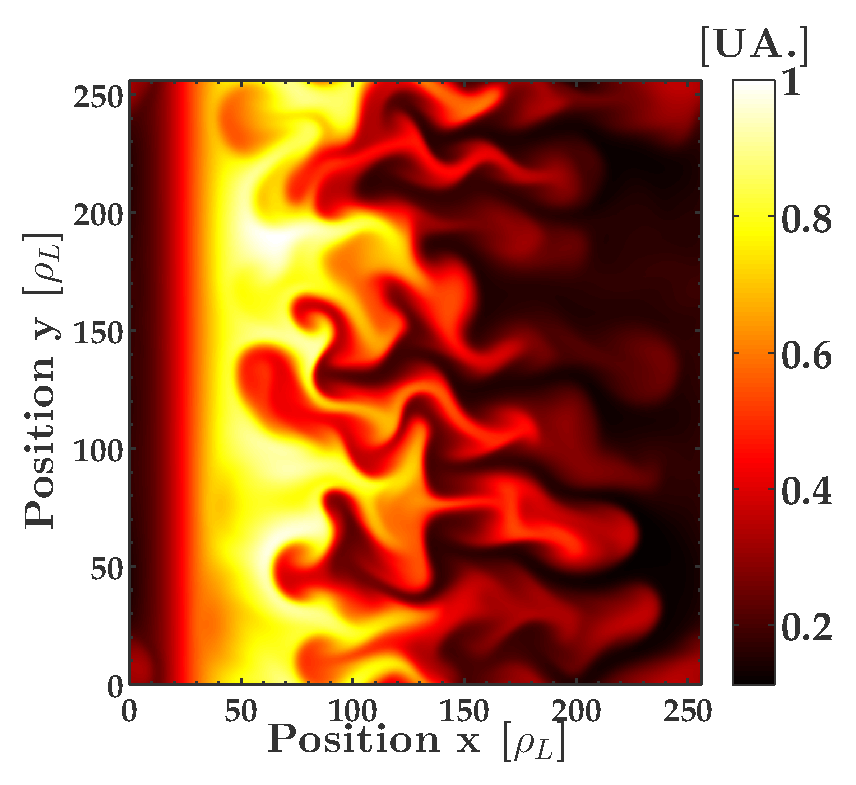
\includegraphics[height=6cm]{figures/2-CarteDensiteBase.eps}}
    \subfigure[]{\label{2-CartePotentielBase}
    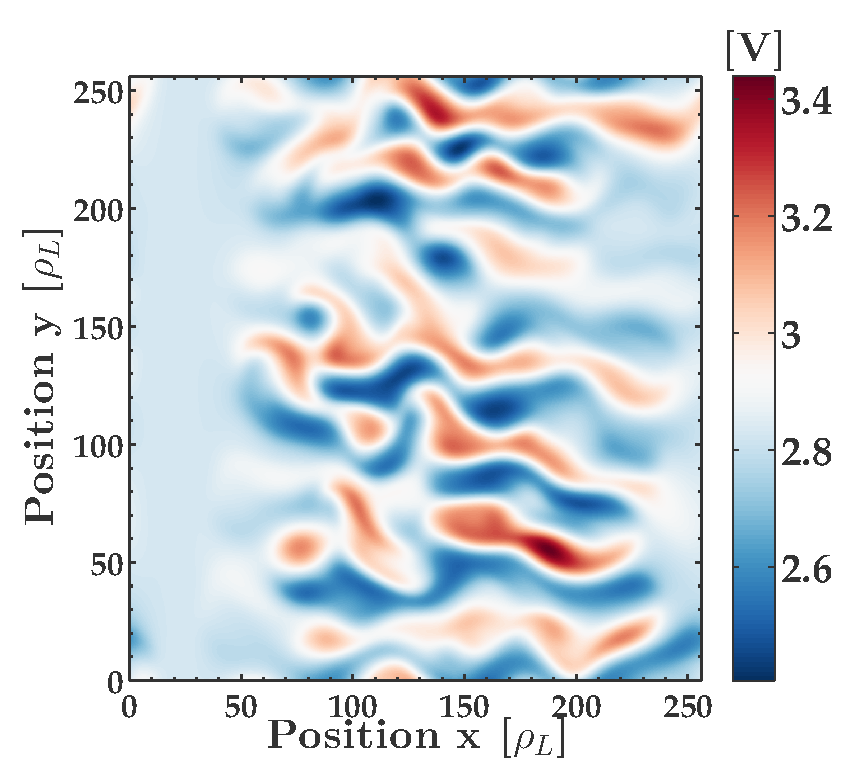
\includegraphics[height=6cm]{figures/2-CartePotentielBase.eps}}
    \caption{Cartes de la densité \subref{2-CarteDensiteBase}~~et du potentiel
    électrostatique
    \subref{2-CartePotentielBase}}
    \label{2-CartesBase}
\end{figure}

\begin{figure}[htbp]
\centering
    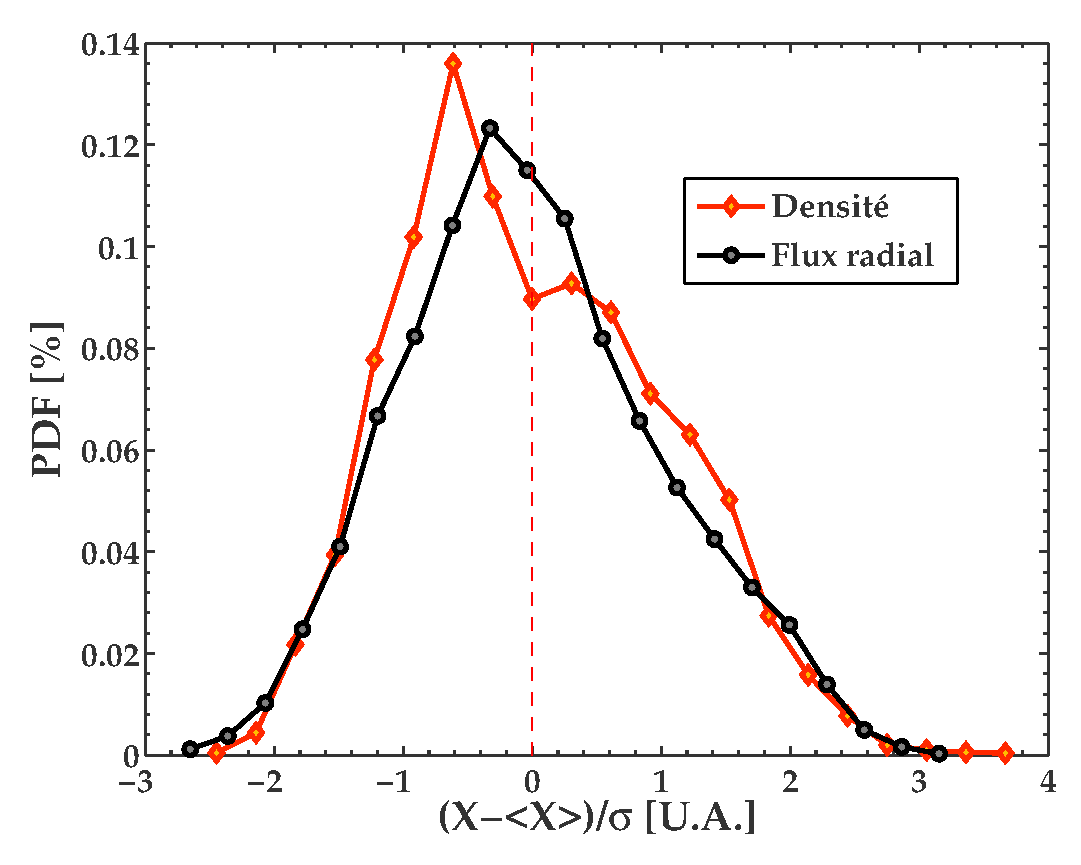
\includegraphics[width=10cm]{figures/2-PDFBase.eps}
    \caption{Densité de probabilité pour la densité et le flux radial}
    \label{2-PDFBase}
\end{figure}


\section{Vers une description des sources d'ions}
L'approche par les vitesses de dérive utilisée pour construire le modèle de TOKAM2D n'est pas 
réellement justifiée dans le cas des sources d'ions. Le modèle suppose tout
d'abord une forte magnétisation des particules limitant le transport transverse,
$v_\perp<<v_\text{th}$, ce qui n'est pas du tout le cas dans les zones faiblement ou non-magnétisées. 

Le code TOKAM2D peut toutefois être complété pour décrire des cas limites de notre étude, \emph{ie.} des plasmas totalement ionisés
confinés par un champ magnétique suffisement intense. Les questions de confinement transverse, d'inhomogénéité du champ 
magnétique et d'influence de la température sont alors utiles pour :
\begin{itemize}
	\item mesurer les approximations faites dans TOKAM2D et leur impact sur le transport transverse dans la SOL
	\item donner un aperçu du transport dans des configurations de type source d'ions, ainsi que des résultats sur les 
	cas limites fortement magnétisés à étudier et comparer.
\end{itemize}
	\subsection{Etude sur les conditions aux limites}
	Les systèmes physiques décrits par les équations fluides sont très sensibles
	aux conditions aux limites imposées par le milieu qui les entoure. Dans les
	plasmas froids ou parallèlement au champ magnétique, cette
	interaction avec les parois est décrite par la théorie des gaines qui donne
	accès à la valeur des flux et des courants, fournissant de ce fait des conditions aux
	limites ayant un sens physique. 
	
	Bien que situation d'une gaine parallèle au champ magnétique soit très mal
	connue (cf. §\ref{1-}) le système doit nécéssairement être fermé, impliquant un
	choix de conditions aux limites de façon arbitraire. Mais avec quel impact sur le
	système? La simplification de TOKAM2D de considérer une géométrie bipériodique
	dans le plan transverse est fondamentalement injustifiée, mais a-t-elle une
	influence sur le transport transverse en soi? Quels sont les effets d'autres
	conditions aux limites courament utilisées?
	
	\begin{figure}[htbp]
\centering
    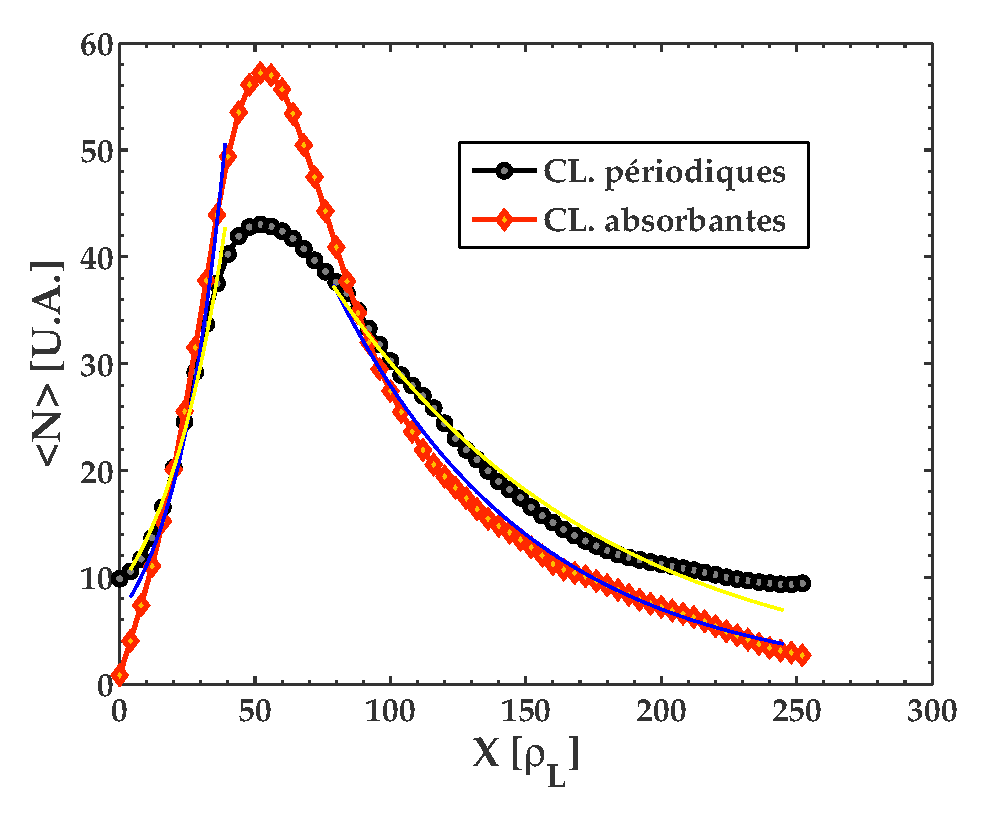
\includegraphics[width=8cm]{figures/2-profileDenNoLimit.eps}
    \caption{Profile de densité pour un cas périodique et un cas
    absorbant\label{2-profileDenNoLimit}}
\end{figure}
\footnotemark{}
\footnotetext{Les conditions aux parois absorbantes}
	
	La prise en compte de conditions aux limites physiques telle que des conditions dérivées du critère de Bohm 
	sont nécéssaires pour décrire correctement la physique du transport dans les plasmas. 
	
	\subsection{Inclusion d'un champ magnétique non uniforme}
	Dans les plasmas de fusions, l'inhomogénéité du champ magnétique est responsable d'une majeure partie du transport turbulent.
	L'inclusion d'un champ magnétique inhomogène en espace a permis d'élargir le domaine de fonctionnalité de TOKAM2D. 
	
	Le cas d'une barrière magnétique montre...
	\begin{figure}
    \centering
    \subfigure[]{\label{2-CarteDensiteMagBarrier}
    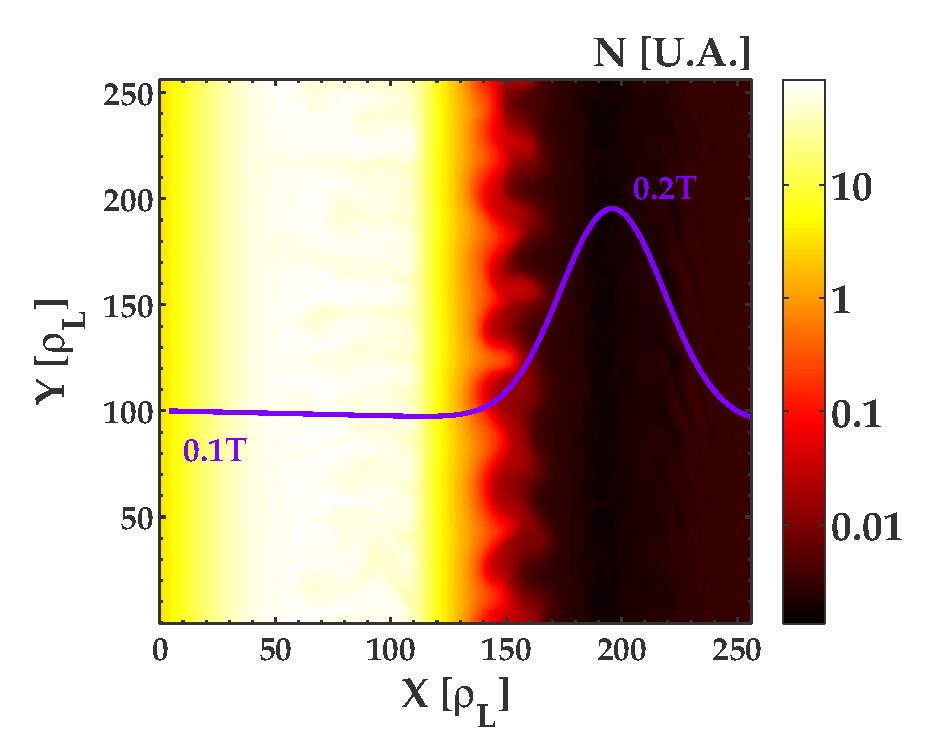
\includegraphics[height=5.8cm]{figures/2-CarteDensiteMagBarrier.eps}}
    \subfigure[]{\label{2-CartePotentielMagBarrier}
    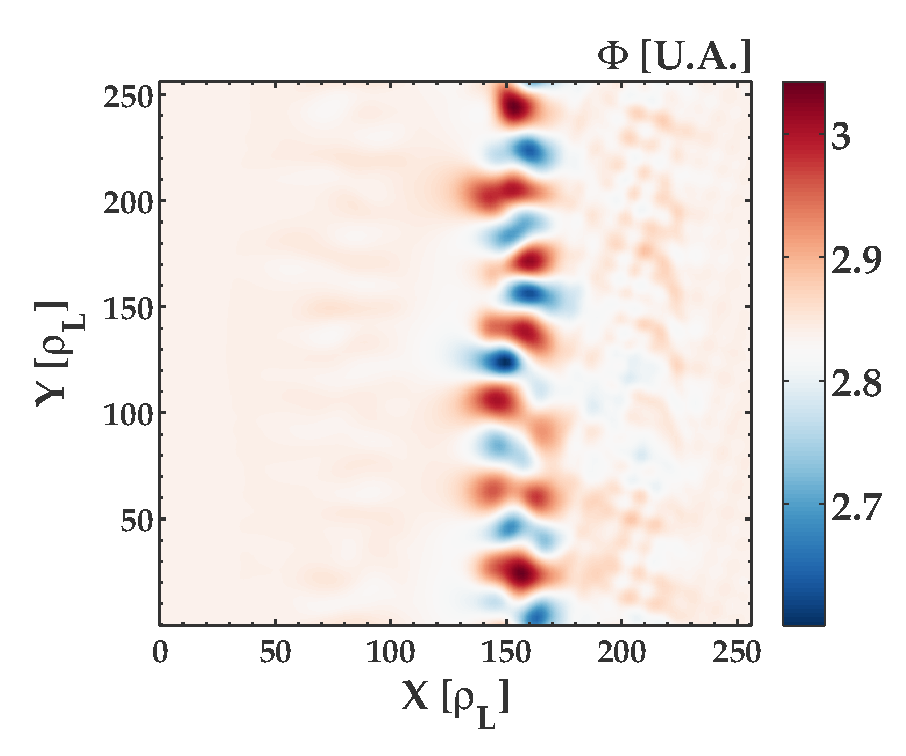
\includegraphics[height=5.8cm]{figures/2-CartePotentielMagBarrier.eps}}
    \caption{Cartes de densité \subref{2-CarteDensiteMagBarrier} et de potentiel
    \subref{2-CartePotentielMagBarrier}}
    \label{2-CartesMagBarrier}
\end{figure}

	
	De très faibles inhomogénéités pouvant être responsable d'une modification non-négligeable du transport transverse, il pourrait 
	être intéressant de poursuivre l'étude dans cette direction.
	
	\subsection{Implémentation de l'équation d'énergie}
	La fermeture isoterme considérée dans le modèle de TOKAM2D est aussi très
	discutable. Le transport transverse dans la SOL est directement lié aux
	variations du potentiel plasma à travers la dérive ExB.  Les effets de la température et de la chaleur deviennent
	non-négligeables dès que $\omega>>\text{?}$. De plus la prise en compte des
	variations spatiales de la température complexifie grandement la relation de
	dispersion du modèle, et pouvant donner lieu à l'apparition d'instabilités différentes de l'interchange.
	Les équations du modèle s'écrivent alors :
	
	\begin{equation}\begin{split}
		\partial_t N + \nabla_\perp\cdot\left(NB^{^{-2}}\mathbf{E}\times\mathbf{B}\right)
		+ \nabla_\perp\cdot\left(B^{^{-2}}\nabla P_e\times\mathbf{B}\right)
		  \\= \sigma_\para N{T_e}^{\text{\textonehalf}} exp({\Lambda-\Delta\Phi/T_e}) 
		 + D_\perp\nabla^2_\perp N + S
		 \end{split}
	\end{equation}
	
	aa
	
	\begin{equation}\begin{split}
			\partial_\text{t}\nabla_\perp^2 \Phi +\nabla_\perp\cdot\left(\nabla_\perp^2 \Phi\frac{\mathbf{E}\times\mathbf{B}}{B^2}\right)
			+ \nabla_\perp\cdot\left(\frac{\nabla P\times\mathbf{B}}{B^2}\right)
			\\= 
		\sigma_\para {T_e}^{\text{\textonehalf}}\left(1-e^{\Lambda-\Delta\Phi/T_e}\right) +\nu_\perp\nabla_\perp^4\Phi
	\end{split}\end{equation}
	
	\begin{figure}
    \centering
    \subfigure[]{\label{2-CarteDensiteWithTe}
    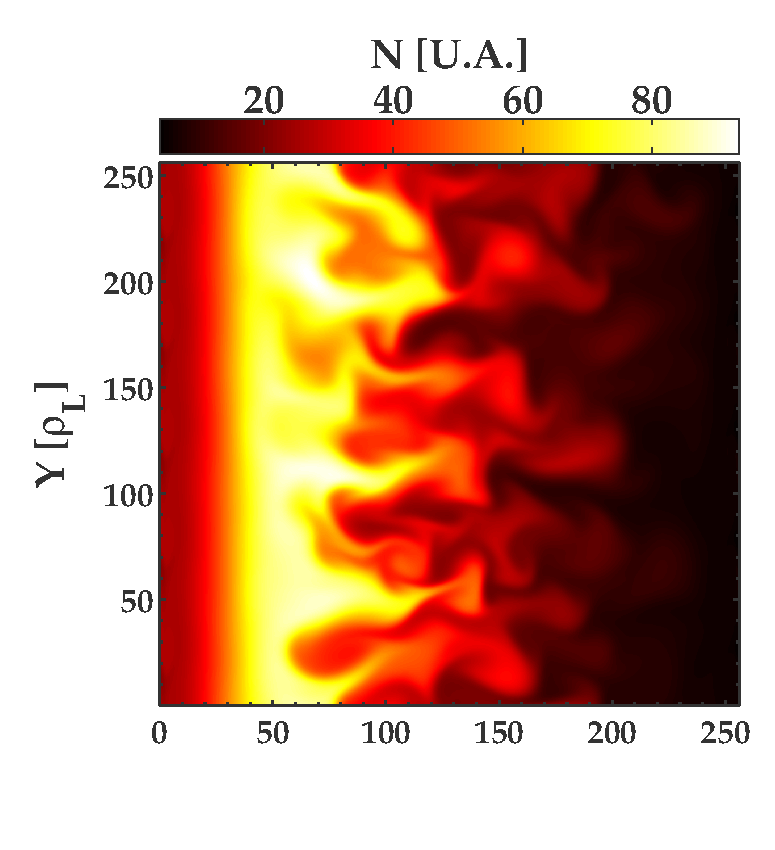
\includegraphics[height=5.75cm]{figures/2-CarteDensiteWhTe.eps}}
    \subfigure[]{\label{2-CartePotentielWithTe}
    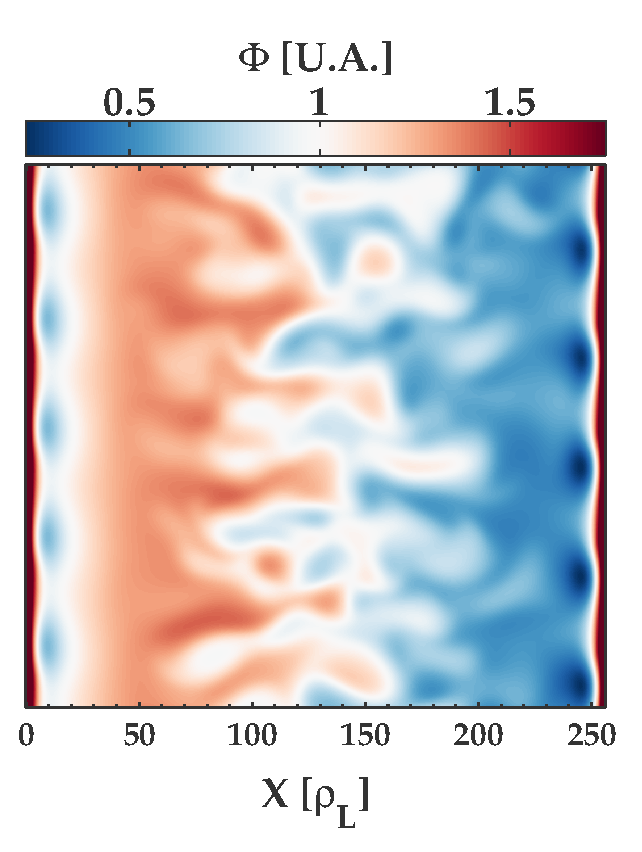
\includegraphics[height=5.75cm]{figures/2-CartePotentielWhTe.eps}}
    \subfigure[]{\label{2-CarteTeWhTe}
    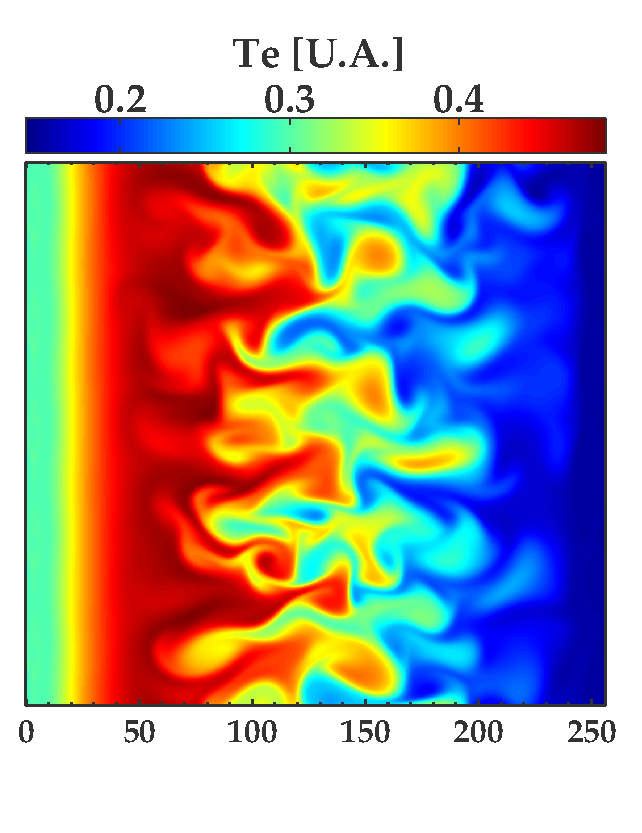
\includegraphics[height=5.75cm]{figures/2-CarteTeWhTe.eps}}
    \caption{Cartes de densité \subref{2-CarteDensiteBase}, de potentiel
    \subref{2-CartePotentielBase} et de température \subref{2-CarteDensiteBase}}
    \label{2-CartesWithTe}
	\end{figure}
	
	\begin{figure}[htbp]
\centering
    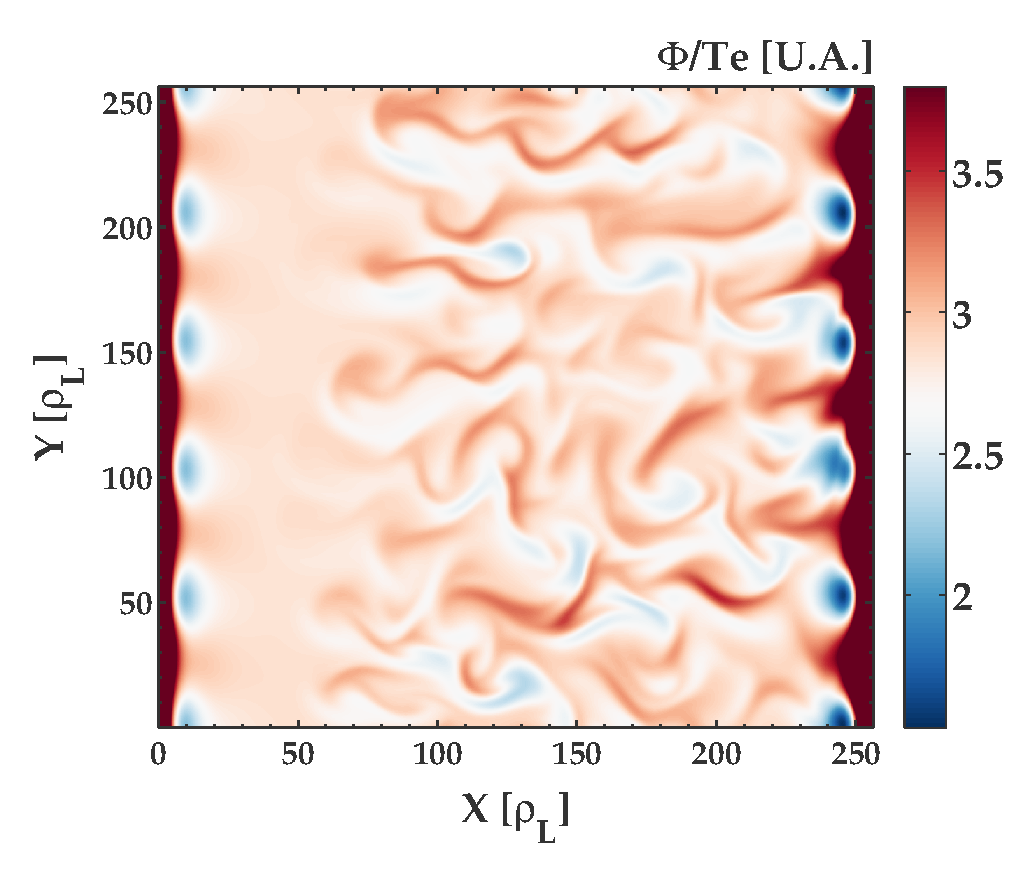
\includegraphics[width=10cm]{figures/2-CartePotentielSurTeWhTedNdx.eps}
    \caption{Carte du potentiel électrostatique rapporté à la température.}
    \label{2-CartePotentielSurTeWhTedNdx}
\end{figure}

	
	\subsubsection{Impact sur le transport transverse}
	
	\begin{figure}[htbp]
    \centering
    \subfigure[]{\label{2-CarteDensiteWhTe}
    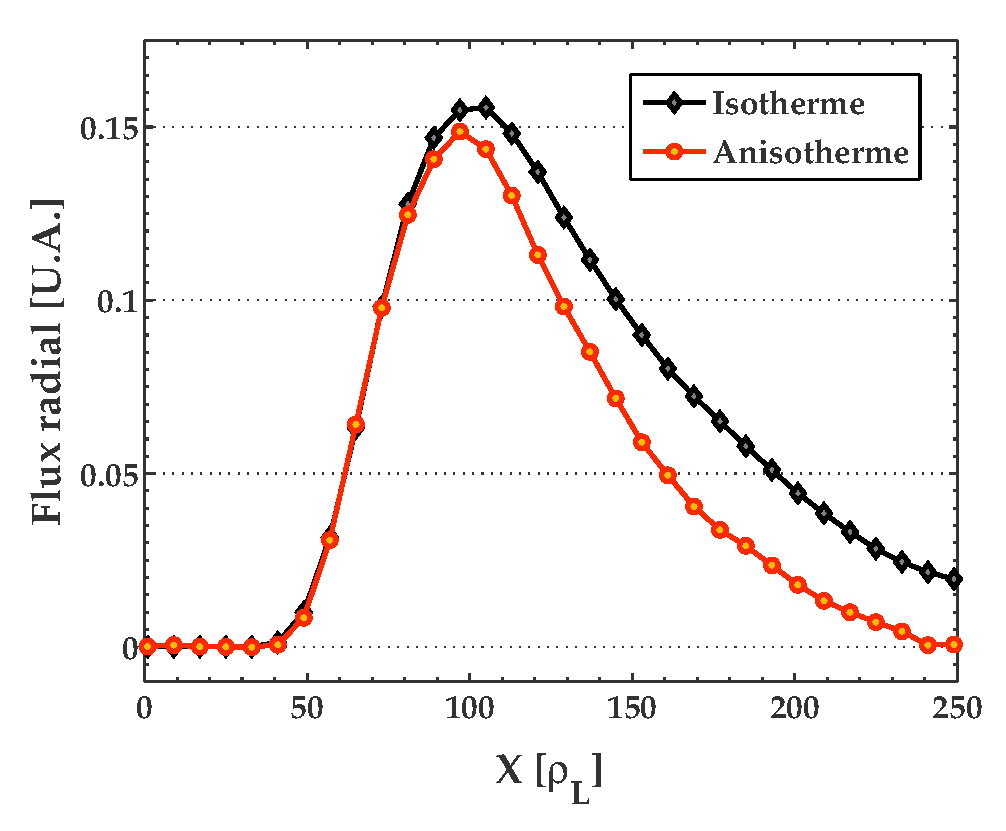
\includegraphics[height=5cm]{figures/2-profileFluxRadialWhTedNdx.eps}}
    \subfigure[]{\label{2-profileFluxRadialWhTedNdx}
    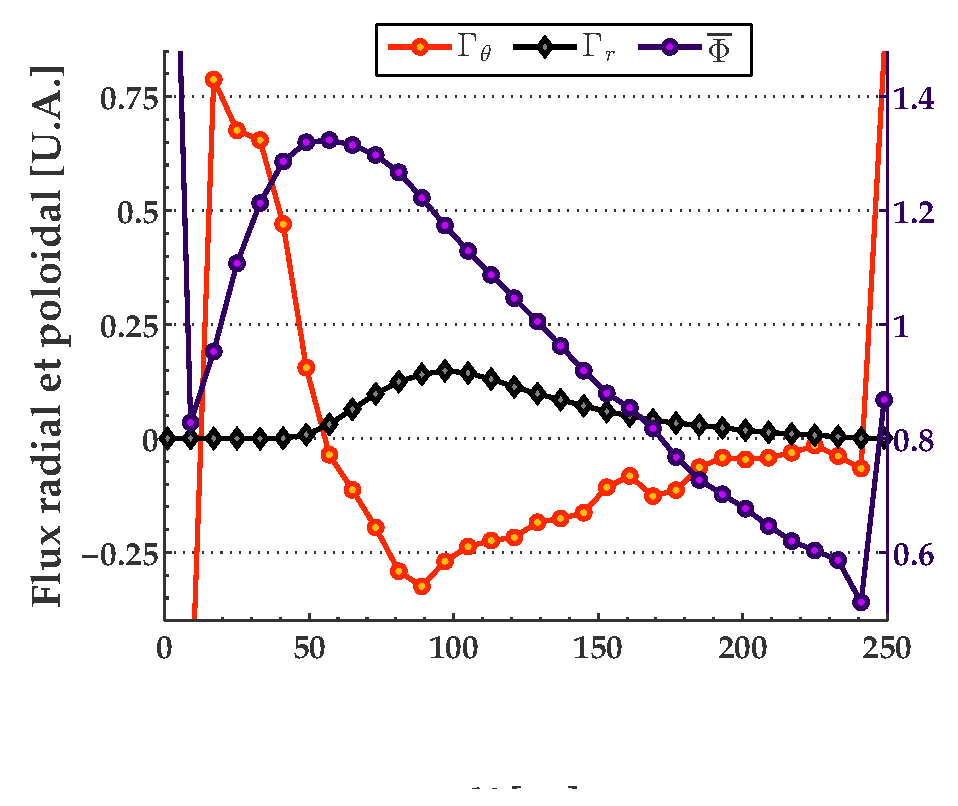
\includegraphics[height=6cm]{figures/2-profileFluxWhTedNdx.eps}}
    \caption{Cartes de densité \subref{2-CarteDensiteWhTe}, de potentiel
    \subref{2-CartePotentielBase} et de température \subref{2-profileFluxWhTedNdx}}
    \label{2-CartesWithTe}
	\end{figure}
	
	\subsubsection{Application au filtre magnétique}
	\begin{figure}[htbp]
    \centering
    \subfigure[]{\label{2-CarteDensiteMagBarrierWhTe}
    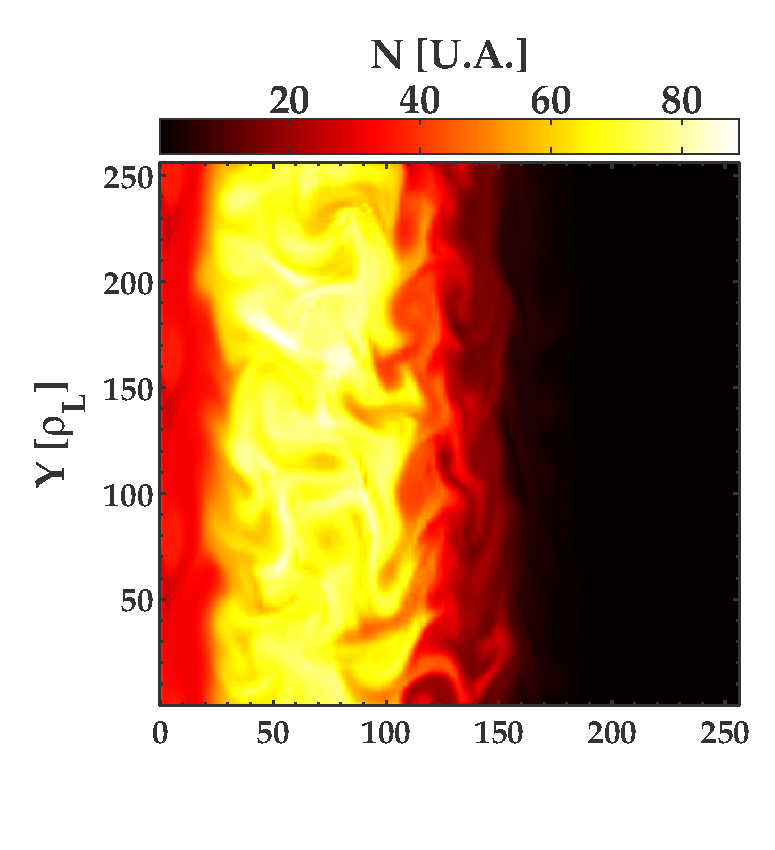
\includegraphics[height=5.75cm]{figures/2-CarteDensiteMagBarrierWhTe.eps}}
    \subfigure[]{\label{2-CartePotentielMagBarrierWhTe}
    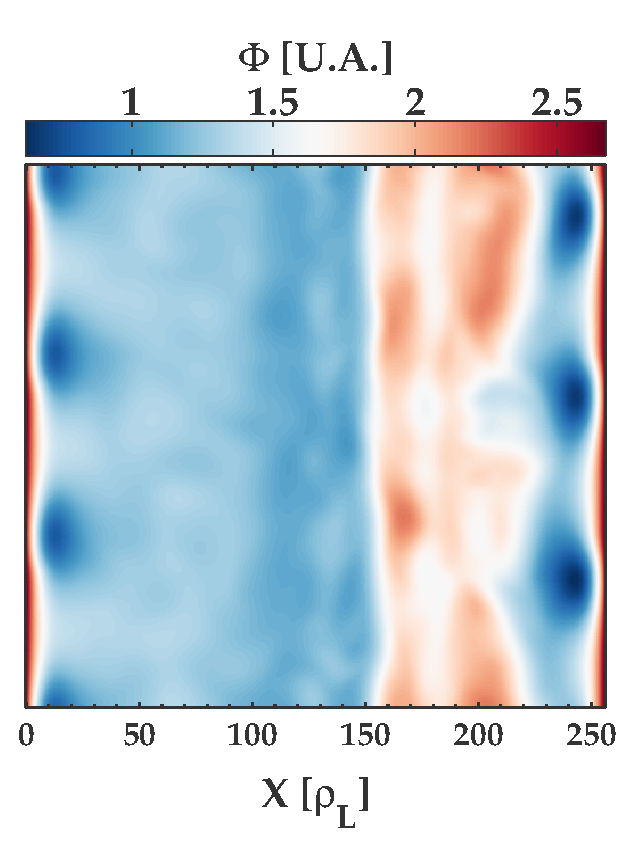
\includegraphics[height=5.75cm]{figures/2-CartePotentielMagBarrierWhTe.eps}}
    \subfigure[]{\label{2-CarteTeMagBarrierWhTe}
    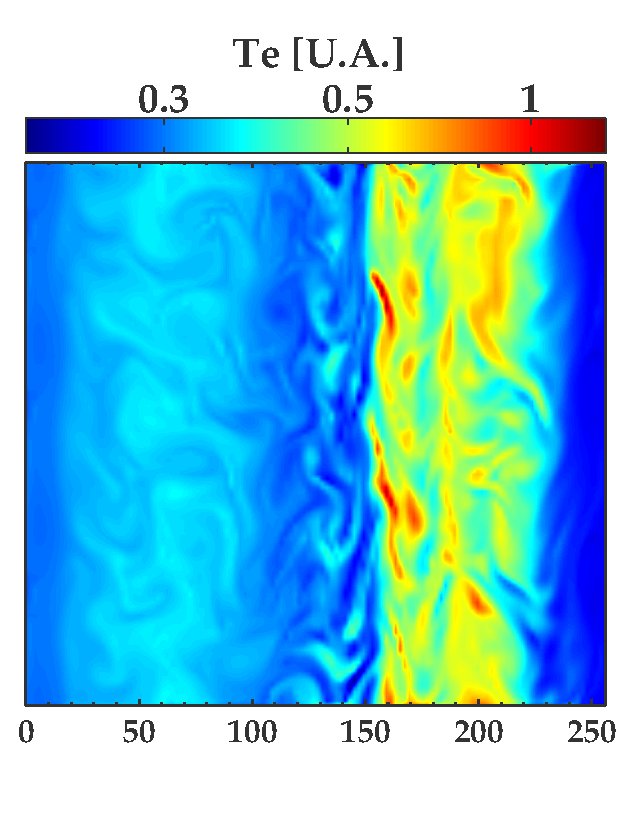
\includegraphics[height=5.75cm]{figures/2-CarteTeMagBarrierWhTe.eps}}
    \caption{Cartes de densité \subref{2-CarteDensiteMagBarrierWhTe}, de potentiel
    \subref{2-CartePotentielMagBarrierWhTe} et de température \subref{2-CarteTeMagBarrierWhTe}}
    \label{2-CartesWithTe}
	\end{figure}
	
	\subsubsection{Simulation d'une colonne de plasma magnétisée}
	
	\begin{figure}[htbp]
    \centering
    \subfigure[]{\label{2-CarteDensiteMagColumn}
    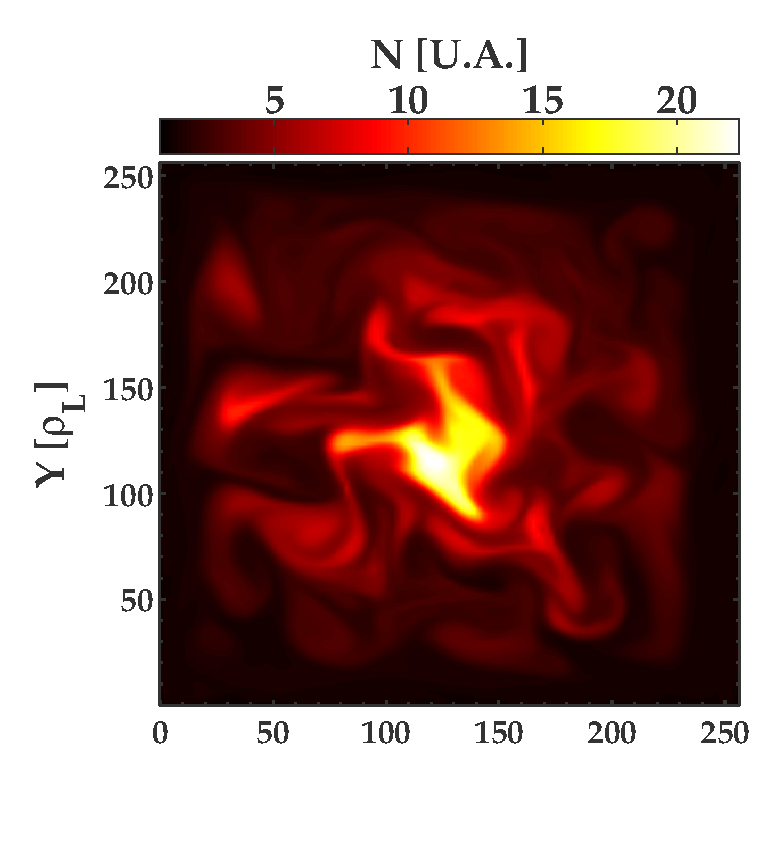
\includegraphics[height=5.75cm]{figures/2-CarteDensiteMagColumn.eps}}
    \subfigure[]{\label{2-CartePotentielMagColumn}
    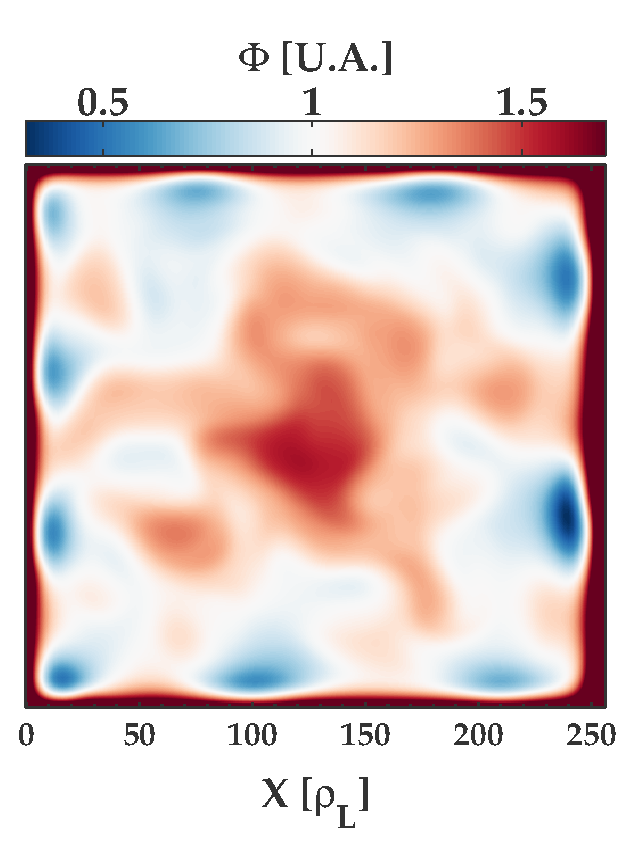
\includegraphics[height=5.75cm]{figures/2-CartePotentielMagColumn.eps}}
    \subfigure[]{\label{2-CarteTeMagColumn}
    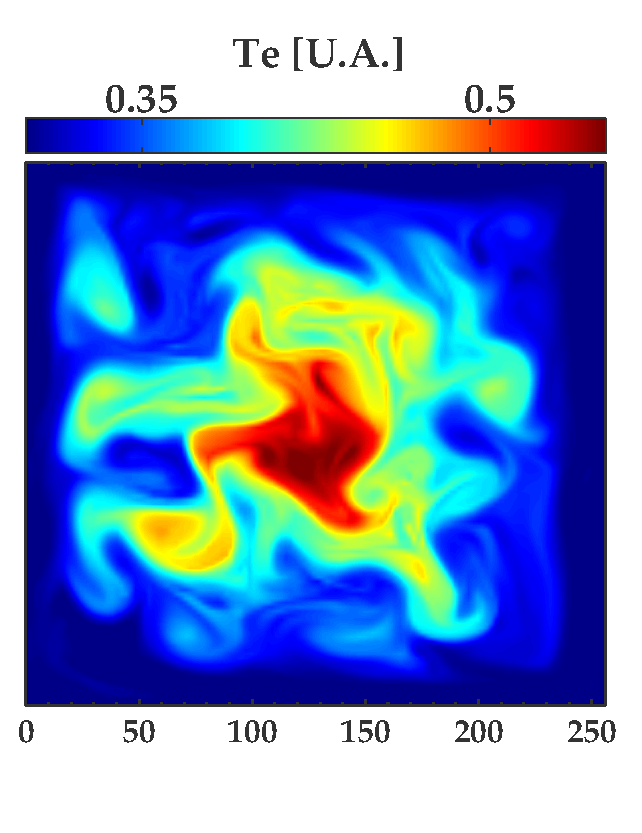
\includegraphics[height=5.75cm]{figures/2-CarteTeMagColumn.eps}}
    \caption{Cartes de densité \subref{2-CarteDensiteMagColumn}, de potentiel
    \subref{2-CartePotentielMagColumn} et de température \subref{2-CarteTeMagColumn}}
    \label{2-CartesWithTe}
	\end{figure}
\section{L'approche par vitesses de dérive pour les plasmas
froids}
\label{vitessesDerivePlasmaFroid}
Les équations de TOKAM2D ne décrivent pas non plus l'intéraction
collisionnelle des particules chargées avec la population neutre, essentielle dans la physique des plasmas froids,
\begin{figure}[htbp]
    \centering
    \subfigure[]{\label{2-CarteDensiteMapl}
    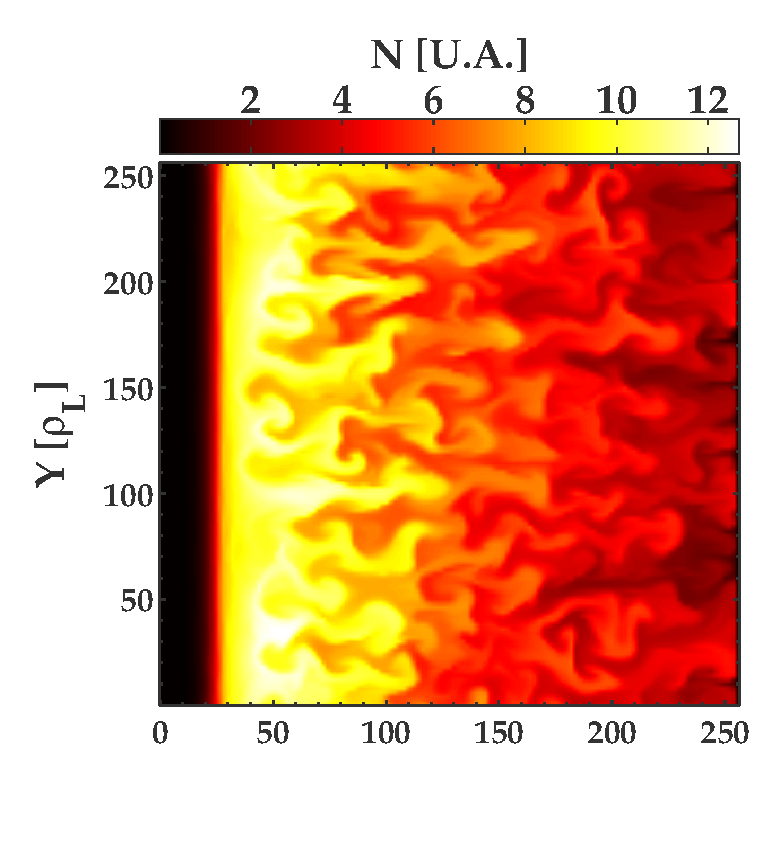
\includegraphics[height=8cm]{figures/2-CarteDensiteMapl.eps}}
    \subfigure[]{\label{2-CartePotentielMapl}
    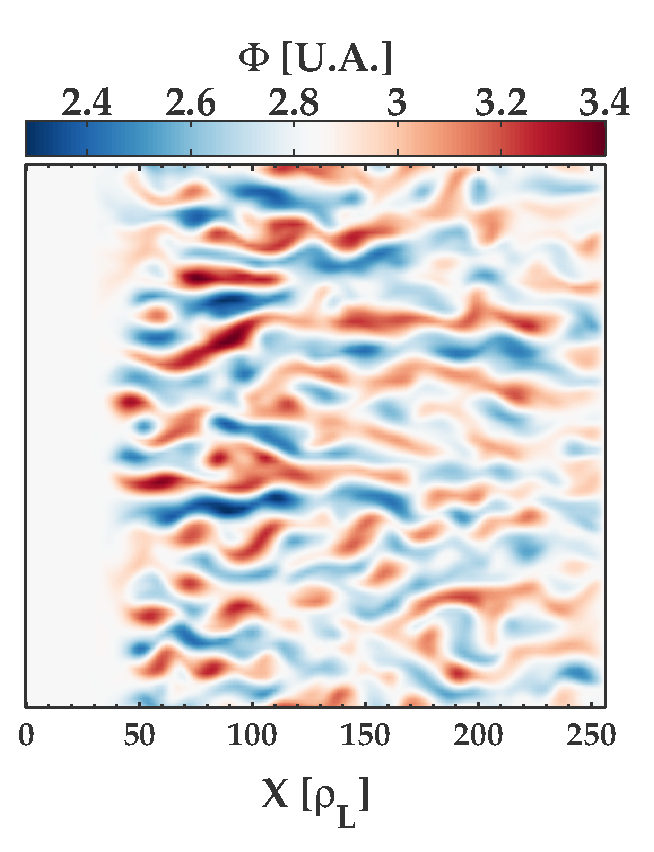
\includegraphics[height=8cm]{figures/2-CartePotentielMapl.eps}}
    \caption{Cartes de densité \subref{2-CarteDensiteMapl}~~et de potentiel
    \subref{2-CartePotentielMapl}}
    \label{2-CartesWithTe}
	\end{figure}
%\bibliographystyle{apalike}
%\bibliography{biblio}

\end{refsection}




